\chapter{Auswertung}
\section{Auswertung der subjektiven Beobachtungen}\label{sec:auswertungSubjektiv}
Im folgenden Abschnitt wird die Auswertung der im vorherigen Kapitel beschriebenen Beobachtungen durchgeführt.
\subsection{Problemstellung}
Nach Abschluss der Beobachtungsphase der Kinder musste nun eine Grundlage geschaffen werden, so dass die Daten, die dabei gesammelt wurden, miteinander vergleichbar werden. Durch die subjektive Beobachtungen der Autoren ist die Vergleichbarkeit nicht gegeben. Daher wurde für die Studienarbeit eine Metrik geschaffen, deren Ziel es war, aus subjektiven Bewertungen Werte zu erhalten, mit welchen besser gerechnet und verglichen werden kann.
\subsection{Entwicklung einer Metrik}
Nachdem alle Daten der Kinder erfasst wurden, sowohl die der Kinder an der \acrshort{dhbw} Karlsruhe als auch an der \acrlong{guc}, wurden alle während der Beobachtung verfassten Formulierungen gesammelt. Dies wurde gemacht, um einen Überblick darüber zu gewinnen, welches Spektrum die Aussagen der Beobachter bildeten. Um aus diesen Formulierungen ein mathematisches Spektrum zu erhalten, mussten zwei Kernfragen beantwortet werden.\\
Zuerst musste geklärt werden, wie feinstufig das Spektrum sein musste. Dies hing davon ab, wie viele verschiedene Formulierungen es bei den einzelnen Antworten gab. Häufig waren jedoch die Antworten sehr überschaubar, oftmals wurde nur ein einzelnes "`yes"' oder "`no"' in den Beobachtungsbögen eingetragen, so dass die Skala, mit der später die Formulierungen in Zahlenwerte umgewandelt werden sollte, nicht sehr fein sein musste. Für die Skala wurde deshalb ein fünfstufiges System definiert. Die Skala beinhaltete einen positiven und einen negativen Teil, welche beide aus je zwei Stufen bestanden. Für die Anschaulichkeit wurde eine zweite Skala geschaffen, so dass es einfacher war, die Werte einzuteilen. Die fünf Stufen, die die Skala zur Anschauung bildeten, waren folgende: --,-,0,+,++. Die Stufe, welche als -- bezeichnet wurde, steht ganz links auf der Skala und bildet damit den schlechtesten Wert. Auf der positiven Seite bildet die Stufe mit der Bezeichnung ++ den höchsten Wert. Mit diesen Bezeichnungen ist es nun möglich, Formulierungen einzuordnen.\\
Da mit diesen Bezeichnungen jedoch noch keine arithmetischen Operationen durchgeführt werden konnte, wurde nun eine zweite fünfstufige Skala definiert. Deren Minimum ist bei 0, was auf der Anschauungs-Skala der Bezeichnung -- entspricht. Das Maximum der Skala liegt bei 4 und ist das Gegenstück zu der Stufe mit der Bezeichnung ++ auf der Anschauungs-Skala. Nachdem die Formulierungen nun in Stufen eingeteilt wurden, konnte mithilfe dieser neuen Skala aus den Beobachtungen Daten gewonnen werden, mit denen nun Vergleiche möglich sind.\\

Die zweite Kernfrage, die sich gestellt hatte, war welche Formulierung in welche Stufe eingeordnet werden muss. Hierfür wurde noch einmal das Spektrum der Beobachtungen analysiert. Durch die bereits erwähnte Häufigkeit der Formulierung "`yes"' wurde diese als Nullpunkt der Skala definiert. Für das linke Ende der Skala wurde "`no"' definiert. Auf der rechten Seite der Skala wurde keine Formulierung definiert, welche das Maximum darstellte.\\
Bei der Einteilung der restlichen Formulierungen wurde danach geschaut, ob eine Formulierung inhaltlich das Kind besser oder schlechter bewerteten als "`yes"'. Sollte es zwischen "`no"' und "`yes"' liegen, so wurde es mit einer Eins bewertet, sollte es besser sein wurde, je nach dem wie sehr positiv die Formulierung war, mit einer Drei oder der Maximalpunktzahl Vier bewertet.\\

Die definierte Skalen sind in der untenstehenden Tabelle definiert. Das Bilden der Skala wurde von einer Studentin der \acrlong{guc} übernommen, welche nur die ihr zur Verfügung gestellten Bewertungsbögen als Grundlage dafür hatte.

\begin{table}[H]
	\centering
	\begin{tabular}{|c|c|c|c|c|}
		\hline
		-- & - & 0 & + & ++ \\
		\hline
		0 & 1 & 2 & 3 & 4 \\
		\hline
	\end{tabular}
	\caption{Definierte Skala nach Reem Ayman}
\end{table}
\subsection{Verifizierung der Metrik}
\begin{figure}[H]
	\centering
	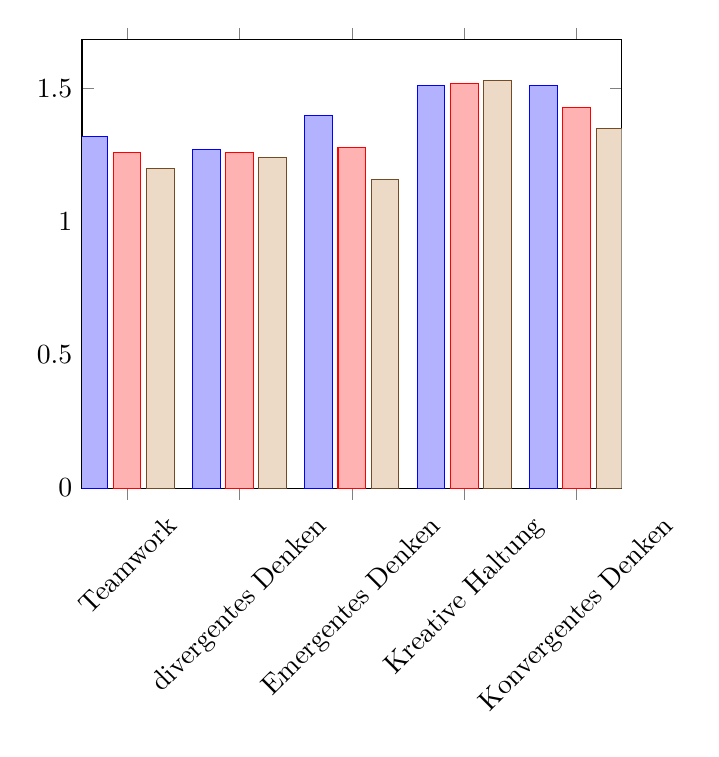
\begin{tikzpicture}
		\begin{axis}[
			ybar,ymin=0,
			symbolic x coords={Teamwork, divergentes Denken, Emergentes Denken, Kreative Haltung, Konvergentes Denken},
			xtick={Teamwork, divergentes Denken, Emergentes Denken, Kreative Haltung, Konvergentes Denken},
			xticklabel style={rotate=45}, legend style={at={(0.5,1)},
				anchor=north,legend columns=-1},
			]
			%Timo
			\addplot coordinates
			{(Teamwork, 1.32)(divergentes Denken,1.27)(Emergentes Denken, 1.4)(Kreative Haltung, 1.51)(Konvergentes Denken,1.51)};\label{diag:Timo}
			%Durchschnitt
			\addplot coordinates
			{(Teamwork, 1.26)(divergentes Denken,1.26)(Emergentes Denken, 1.28)(Kreative Haltung, 1.52)(Konvergentes Denken,1.43)}; \label{diag:average}
			%Reem
			\addplot coordinates
			{(Teamwork, 1.2)(divergentes Denken,1.24)(Emergentes Denken, 1.16)(Kreative Haltung, 1.53)(Konvergentes Denken,1.35)};\label{diag:Reem}
			
		\end{axis}
	\end{tikzpicture}

	\caption[Durchschnittliche Bewertung der Formulierungen]{Durchschnittliche Bewertung der Formulierungen zweier unabhängig voneinander bewertenden Person}
	\label{img:verificationMetric}
\end{figure}
Abbildung \ref{img:verificationMetric} zeigt wie eindeutig die von Reem Ayman definierte Metrik ist. Je weiter die beiden Balken von Timo Steidinger und Reem Ayman auseinanderliegen, umso schlechter funktioniert die Skala. Die genauen Differenzen aus der obigen Abbildung sind als durchschnittliche Abweichung in Tabelle \ref{tab:differences} aufgeführt.

\begin{table}[H]
	\centering
	\begin{tabular}{|
			>{\columncolor[HTML]{C0C0C0}}l |c|}
		\hline
		Kategorie & \multicolumn{1}{l|}{\cellcolor[HTML]{C0C0C0}durchschnittliche Abweichung} \\ \hline
		Teamwork            & 0.12 \\ \hline
		Divergentes Denken  & 0.03 \\ \hline
		Emergentes Denken   & 0.24 \\ \hline
		Kreative Haltung    & 0.02 \\ \hline
		Konvergentes Denken & 0.16 \\ \hline
		Mittlere Abweichung & 0.10 \\ \hline
	\end{tabular}
	\caption{Durchschnittliche Abweichung der beiden Bewertungen}
	\label{tab:differences}
\end{table}

\begin{table}[H]
	\centering
	\begin{tabular}{l|l|l|l|l|l|l|}
		\cline{2-7}
		&
		\cellcolor[HTML]{C0C0C0}0 &
		\cellcolor[HTML]{C0C0C0}1 &
		\cellcolor[HTML]{C0C0C0}2 &
		\cellcolor[HTML]{C0C0C0}3 &
		\cellcolor[HTML]{C0C0C0}4 &
		\cellcolor[HTML]{C0C0C0}Summe \\ \hline
		\multicolumn{1}{|l|}{\cellcolor[HTML]{C0C0C0}0}     & 286 & 43  & 6   & 2   & 0  & 337 \\ \hline
		\multicolumn{1}{|l|}{\cellcolor[HTML]{C0C0C0}1}     & 38  & 100 & 35  & 10  & 1  & 184 \\ \hline
		\multicolumn{1}{|l|}{\cellcolor[HTML]{C0C0C0}2}     & 2   & 10  & 224 & 72  & 9  & 317 \\ \hline
		\multicolumn{1}{|l|}{\cellcolor[HTML]{C0C0C0}3}     & 1   & 5   & 77  & 70  & 26 & 179 \\ \hline
		\multicolumn{1}{|l|}{\cellcolor[HTML]{C0C0C0}4}     & 0   & 0   & 0   & 1   & 2  & 3   \\ \hline
		\multicolumn{1}{|l|}{\cellcolor[HTML]{C0C0C0}Summe} & 327 & 158 & 342 & 155 & 38 & 682 \\ \hline
	\end{tabular}
	\caption{Übereinstimmungsmatrix}
	\label{tab:agreement}
\end{table}

 
 Insgesamt wurden 1020 Bewertungen durch Zahlen ersetzt. Die Zahlen in der Tabelle \ref{tab:agreement} zeigen die Übereinstimmungsmatrix nach Abschluss der Bewertungen. Diese Matrix dient zur Verifikation der Bewertungen aus dem vorherigen Kapitel. Dazu wird die sogenannte Interrater-Reliabilität ermittelt. Da für diese Arbeit zwei verschiedene Bewerter die Bewertung durchgeführt haben, wird das Ergebnis der Interrater-Reliabilität nach Jacob Cohen berechnet:\cite{cohen_1960}\\
 
 \begin{figure}[H]
 	\centering
 	\begin{equation}
 		\kappa = \frac{p_{0} - p_{c}}{1 - p_{c}}
 	\end{equation}
 	\begin{equation}
 		p_{0} = (682/1020) = 0.67
 	\end{equation}
 	\begin{equation}
 		p_{e} = (0.32)^{2} + (0.15)^{2} + (0.34)^{2} + (0.15)^{2} + (0.04)^{2} =  0.26
 	\end{equation}
 	\begin{equation}
 		\kappa = \frac{0.67 - 0.26}{1 - 0.26} = 0.74
 	\end{equation}
 	\caption{Berechnung der Interrater-Reliabilität}
 	\label{img:calc}
 \end{figure}

Mithilfe von Kappa kann nun bewertet werden, wie gut die entwickelte Metrik ist. Dazu wird die Bewertung von Kappa nach \citeauthor{Landis77} verwendet. Diese besagt, ein Kappa kleiner als 0 ist ein \glqq Poor Agreement\grqq, ein Kappa zwischen 0.00 und 0.2 gilt als eine leichte Übereinstimmung. Ein Kappa, welches zwischen 0.21 und 0.4 liegt, wird als \glqq Fair Agreement\grqq bezeichnet und sobald der Wert zwischen 0.41 und 0.6 liegt, wird von einer moderaten Übereinstimmung gesprochen. Das Kappa des oben definierten Schemas wird nach \citeauthor{Landis77} als ein \glqq Substantial Agreement\grqq bezeichnet, da es im Bereich von 0.61 und 0.8 liegt, wie die Berechnung oben zeigt. Sollte der Wert des Kappas zwischen 0.81 und 1.00 liegen, so wird von einer fast perfekten Übereinstimmung gesprochen.\\
\noindent
\cite{Landis77}

\section{Entwicklung der Kinder}
\subsection{Jonas}

\begin{figure}[H]
	\centering
	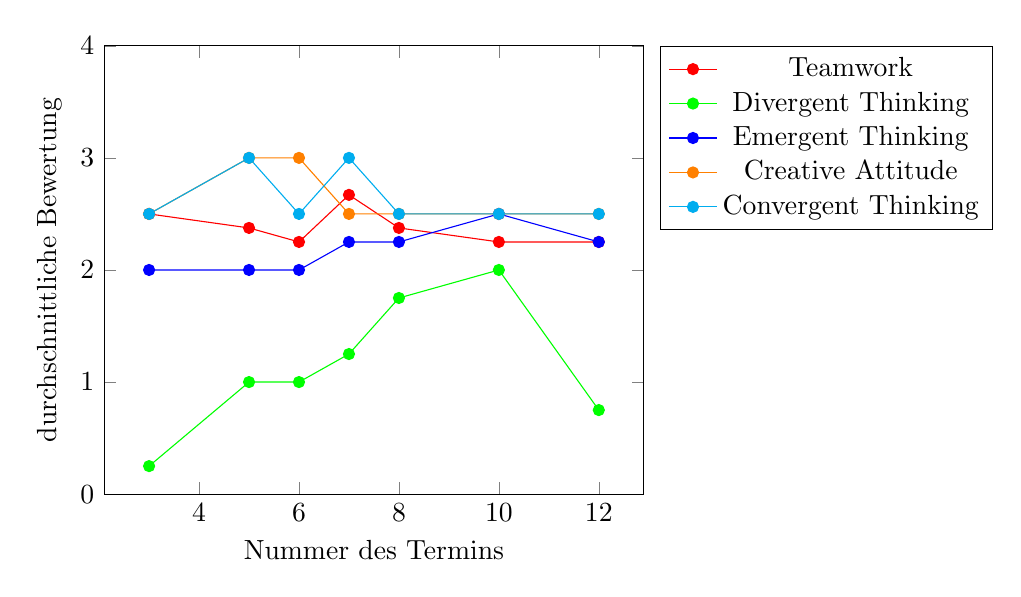
\begin{tikzpicture}
		\begin{axis}[legend pos=outer north east, ymin = 0, ymax = 4,xlabel={Nummer des Termins},ylabel={durchschnittliche Bewertung}]
			\addplot[mark=*,red]
			coordinates {
				(3,2.5) (5,2.375) (6,2.25) (7,2.67) (8,2.375) (10,2.25) (12,2.25)
			};
			\addlegendentry{Teamwork}
			\addplot[mark=*, green]
			coordinates {
				(3,0.25) (5,1) (6,1) (7,1.25) (8,1.75) (10,2) (12,0.75)
			};
			\addlegendentry{Divergent Thinking}
			\addplot[mark=*, blue]
			coordinates {
				(3,2) (5,2) (6,2) (7,2.25) (8,2.25) (10,2.5) (12,2.25)
			};
			\addlegendentry{Emergent Thinking}
			\addplot[mark=*, orange]
			coordinates {
				(3,2.5) (5,3) (6,3) (7,2.5) (8,2.5) (10,2.5) (12,2.5)
			};
			\addlegendentry{Creative Attitude}
			\addplot[mark=*,cyan]
			coordinates {
				(3,2.5) (5,3) (6,2.5) (7,3) (8,2.5) (10,2.5) (12,2.5)
			};
			\addlegendentry{Convergent Thinking}
		\end{axis}
	\end{tikzpicture}
	\caption{Entwicklung von Jonas}
	\label{img:jonasDevelopment}	
\end{figure}

Zu Beginn der Termine an der DHBW Karlsruhe zeigte Jonas wie in Abbildung \ref{img:jonasDevelopment} dargestellt bereits ein hohes Maß an Teamwork. Seine Werte lagen meist um den Wert von 2.5, welches im Vergleich zu anderen Kindern ein sehr guter Wert ist. Jonas zeigte in seinem Verhalten im Team große Konstanz, große Abweichungen sind nur sehr selten. Dies kann mehrere Gründe haben, welche sich beide auf seinen Teampartner Mario beziehen. Der erste Grund ist das Alter und die Beziehung der beiden Kinder zueinander. Mario und auch Jonas besuchen die gleiche Schule und Klasse, weshalb sie sich untereinander besser verstehen. Zudem sind beide Kinder männlich und haben etwa das gleiche Alter. Die beiden Faktoren können eine Rolle in der Konstanz spielen, da beide sehr oft zusammenarbeiteten. Der zweite Grund ist der Persönlichkeitstyp. Dies wird aber in Kapitel \ref{sec:personalityAndDevelopment} noch genauer aufgeführt.\\
Etwas schlechter fällt dafür das divergente Denken des Kindes aus. Hier erreicht Jonas ein Maximum von 2.0, welches im Vergleich innerhalb der Gruppe ein sehr guter Wert ist. Für diesen Bereich der Beobachtungen ist bei Jonas eine sehr gute Entwicklung sichtbar. Er entwickelte sich von einer sehr schlechten Bewertung zu einer der besten Bewertungen, die im Verlaufe der Termine dokumentiert wurden. Es liegt nahe, dass Jonas sich über die Zeit mehr und mehr mit dem Thema vertraut gemacht hatte, auch außerhalb der Kurse. Dadurch fiel ihm einerseits der Umgang, als auch das Generieren von Ideen im Bezug auf die Projekte innerhalb der Kurse leichter.\\
Ebenfalls sehr gut waren Jonas Fähigkeiten im Bereich des emergenten Denkens. Mit Werten ab 2.0 ist er auch hier an der Spitze im Vergleich zum Rest des Kurses. Über den Zeitraum der Kurse ist hier sogar eine leichte Entwicklung zu sehen, so dass sogar Spitzenwerte von 2.5 erreicht wurden. Grund hierfür kann auch wieder die Beschäftigung mit dem Thema außerhalb sein, da er hierdurch durch das Bauen von verschiedenen Modellen auf allgemeinere Modelle  schließen konnte, wodurch in den Beobachtungsbögen sehr gute Beobachtungen notiert werden konnten.\\
Jonas Haltung gegenüber Kreativität ist ebenfalls überdurchschnittlich. Während den Veranstaltungen zeigte er oft ein hohes Maß an Kreativität sowie an Offenheit, weshalb seine Werte hier die Marke von 2.5 nicht unterschritten. Bis auf zwei Termine war Jonas Haltung sehr konstant, was an der guten Bewertung durch die Autoren liegen kann. Die Notizen zeigten bereits ein sehr gutes Verhalten, so dass nach oben nur wenig Potenzial zur Verbesserung war, jedoch es nicht ganz für die maximale Bewertung gereicht hat. Die Entwicklung, um den letzten Schritt auf eine volle Punktzahl zu erreichen, hat gefehlt, so dass zwar jedes Mal eine hohe Bewertung notiert wurde, aber keine wirkliche Entwicklung zu sehen ist. Generell kann sowohl für Jonas als auch für die anderen Kinder gesagt werden, dass die Bewertung der Kinder nicht komplett linear erfolgt, sondern eher die Form einer Sättigungskurve annimmt. Dies bedeutet, dass für relativ wenig Entwicklung eine höhere Punktzahl vergeben wurde, jedoch ab einem bestimmten Wert ein größerer Fortschritt sichtbar sein muss, damit die Autoren in den Notizen einen wirklichen Fortschritt notierten.\\
Zu guter Letzt ist auch die Fähigkeit des konvergenten Denkens bei Jonas sehr ausgeprägt, so dass er mehrmals die Spitzenwerte von 3.0 erreichte. Auch hier zeigt sich wieder die Konstanz, dessen Ursprung vermutlich ebenfalls in der Nichtlinearität der Bewertungen liegt. Daher besteht die Möglichkeit, dass kleine Fortschritte gemacht wurden, diese jedoch durch die subjektiven Eindrücke der Beobachter weggefallen sind.
    

\subsection{Mario}
\begin{figure}[H]
	\centering
	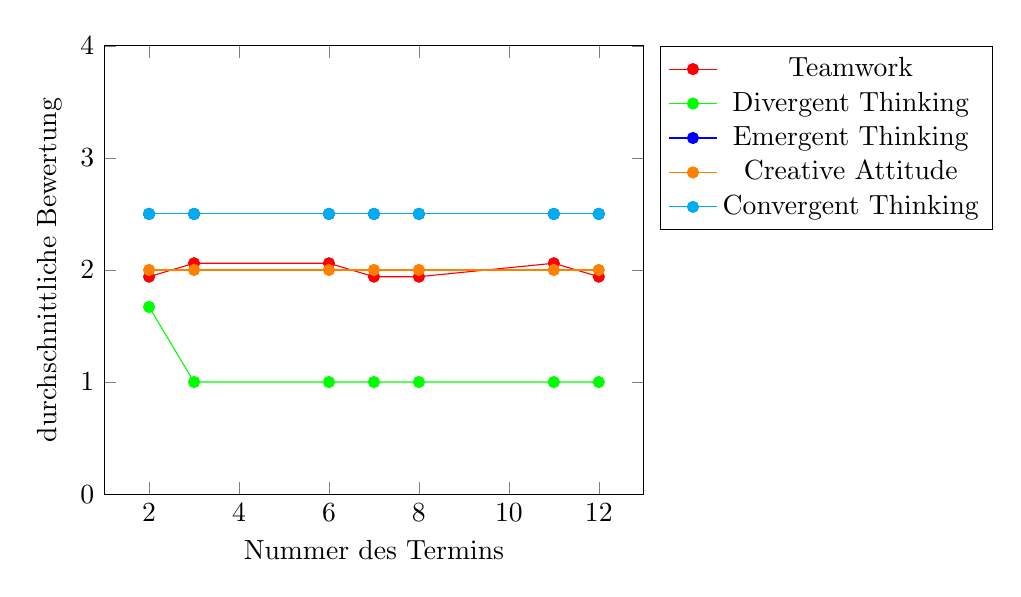
\begin{tikzpicture}
		\begin{axis}[legend pos=outer north east, ymin = 0, ymax = 4,xlabel={Nummer des Termins},ylabel={durchschnittliche Bewertung}]
			\addplot[mark=*, red]
			coordinates {
				(2,1.94)(3,2.06)(6,2.06)(7,1.94)(8,1.94)(11,2.06)(12,1.94)
			};
			\addlegendentry{Teamwork}
			\addplot[mark=*, green]
			coordinates {
				(2,1.67)(3,1)(6,1)(7,1)(8,1)(11,1)(12,1)
			};
			\addlegendentry{Divergent Thinking}
			\addplot[mark=*, blue]
			coordinates {
				(2,2.5)(3,2.5)(6,2.5)(7,2.5)(8,2.5)(11,2.5)(12,2.5)
			};
			\addlegendentry{Emergent Thinking}
			\addplot[mark=*, orange]
			coordinates {
				(2,2)(3,2)(6,2)(7,2)(8,2)(11,2)(12,2)
			};
			\addlegendentry{Creative Attitude}
			\addplot[mark=*, cyan]
			coordinates {
				(2,2.5)(3,2.5)(6,2.5)(7,2.5)(8,2.5)(11,2.5)(12,2.5)
			};
			\addlegendentry{Convergent Thinking}
		\end{axis}
	\end{tikzpicture}
	\caption{Entwicklung von Mario}
	\label{img:marioDevelopment}
	
\end{figure}

Mario zeigte im Verlauf der Termine sehr viel Konstanz. Seine Werte lagen in fast allen Bereichen in einem sehr guten Bereich, weshalb einerseits bei der Fähigkeit des Teamworks wie bereits bei Jonas Beziehung und Alter sowie Persönlichkeitstyp eine Rolle spielen, als auch die bereits angesprochene Nichtlinearität. Diese kann allerdings bei den Kindern unterschiedlich stark ausgeprägt sein. Für Mario ist jedoch in keinem der in Abbildung \ref{img:marioDevelopment} dargestellten Bereiche eine Verbesserung zu notieren.

\subsection{Sara}
\begin{figure}[H]
	\centering
	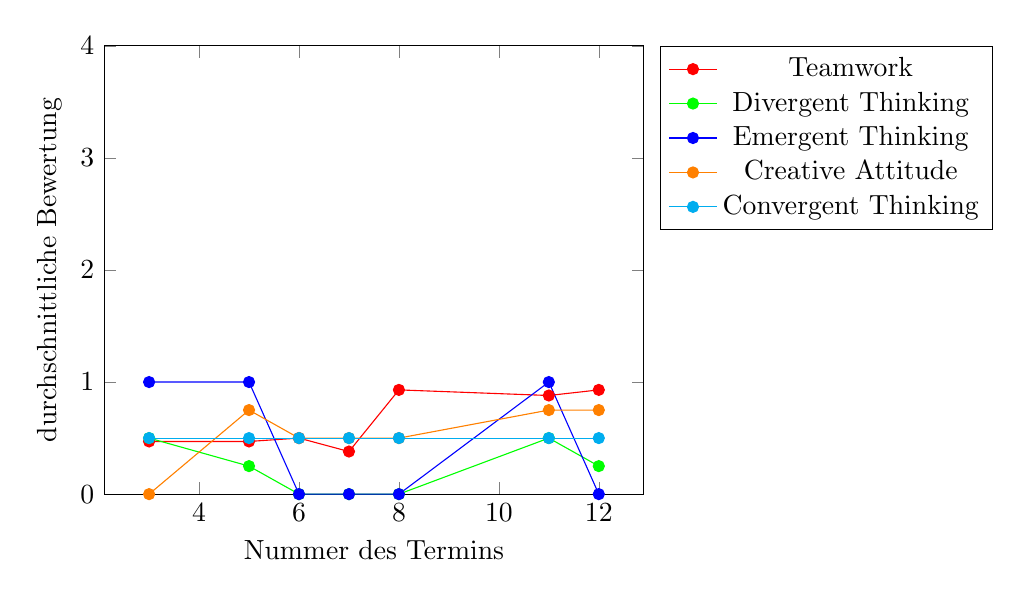
\begin{tikzpicture}
		\begin{axis}[legend pos=outer north east, ymin = 0, ymax = 4,xlabel={Nummer des Termins},ylabel={durchschnittliche Bewertung}]
			\addplot[mark=*, red]
			coordinates {
				(3,.47) (5,.47) (6,.5) (7,.38) (8,0.93) (11,.88) (12,.93)
			};
			\addlegendentry{Teamwork}
			\addplot[mark=*, green]
			coordinates {
				(3,.5) (5,.25) (6,0) (7,0) (8,0) (11,.5) (12,.25)
			};
			\addlegendentry{Divergent Thinking}
			\addplot[mark=*, blue]
			coordinates {
				(3,1) (5,1) (6,0) (7,0) (8,0) (11,1) (12,0)
			};
			\addlegendentry{Emergent Thinking}
			\addplot[mark=*, orange]
			coordinates {
				(3,0) (5,.75) (6,.5) (7,.5) (8,.5) (11,.75) (12,.75)
			};
			\addlegendentry{Creative Attitude}
			\addplot[mark=*, cyan]
			coordinates {
				(3,.5) (5,.5) (6,.5) (7,.5) (8,.5) (11,.5) (12,.5)
			};
			\addlegendentry{Convergent Thinking}
		\end{axis}
	\end{tikzpicture}
	\caption{Entwicklung von Sara}
	\label{img:saraDevelopment}
\end{figure}
Saras Teamfähigkeit lag im Verlaufe der Kurse immer unter dem Durchschnitt, ihre Werte lagen immer unter dem Wert von 1.0. Allerdings lässt sich bei ihr eine positive Entwicklung dokumentieren. So verbessert sich ihre Bewertung der Teamfähigkeit um fast das Doppelte. Dies kann mit der Dauer des Projekts begründet werden. Aus den Notizen kann entnommen werden, dass Sara ein sehr schüchternes Mädchen ist. Allerdings findet sie sich im Laufe der Zeit immer besser in die Gruppe ein, zeigt hier und dort, dass sie auch ein wenig offener sein kann. Die Entwicklung von Sara ist zwar eine der besten Entwicklungen im gesamten Kurs, jedoch bleiben ihre Spitzenwerte im Vergleich zu den anderen Kindern deutlich zurück.\\
Im Bereich des divergenten Denkens schnitt Sara nicht besonders gut ab, hier vermerkten die Beobachter sogar Notizen, welche zu einer Bewertung von 0 führten. Dies war jedoch keine Ausnahme, sondern in einigen Terminen der Fall. Auch hier spielt vermutlich die Schüchternheit von Sara eine Rolle. Für sie wird es vermutlich sehr viel Überwindung gekostet haben, vor der Gruppe zu reden. Da deshalb nur wenig bis keine Wortmeldungen von ihr kamen, konnte dementsprechend auch nur eine sehr schlechte Bewertung für sie notiert werden. Ein zweiter Grund kann die Herkunft von Sara sein. Die genaue Herkunft ist unbekannt, jedoch war auch außerhalb der Gruppenbesprechungen die sprachliche Barriere eine große Hürde für sie. So fehlten häufiger Ausdrücke und Worte, um Gedankengänge und Ideen beschreiben zu können.\\
Ein ähnliches Bild zeigte sich auch bei dem Verlauf der Bewertung ihres emergenten Denkens. Zwar erreichte sie hin und wieder Werte von 1.0 als ihre Spitzenwerte, jedoch damit deutlich unter den Spitzenwerten der anderen Kinder. Auch hier mussten die Autoren bei der Bewertung Sara 0 Punkte geben, so dass über die Hälfte der Termine bei ihr mit null Punkten dokumentiert wurden.\\
Eine positive Entwicklung zeigte sich dagegen bei der Kreativität, welche Sara an den Tag legte. Zwar liegen auch hier wieder die Werte unter dem Durchschnitt des Kurses, jedoch verbesserte sie sich von einer Bewertung mit null Punkten auf einen Maximalwert von 0.75 Punkten. Hier ist vermutlich wieder die Dauer des Projekts ein wichtiger Grund, da sie sich im Verlaufe der Kurse mit den Themen vertraut gemacht hatte und hin und wieder auch einmal kleine Momente der Offenheit und Fantasie. Diese Momente waren zwar nicht sehr groß, aber trotz dessen zeigte sich bei ihr ein positiver Trend.

\subsection{Benny}
\begin{figure}[H]
	\centering
	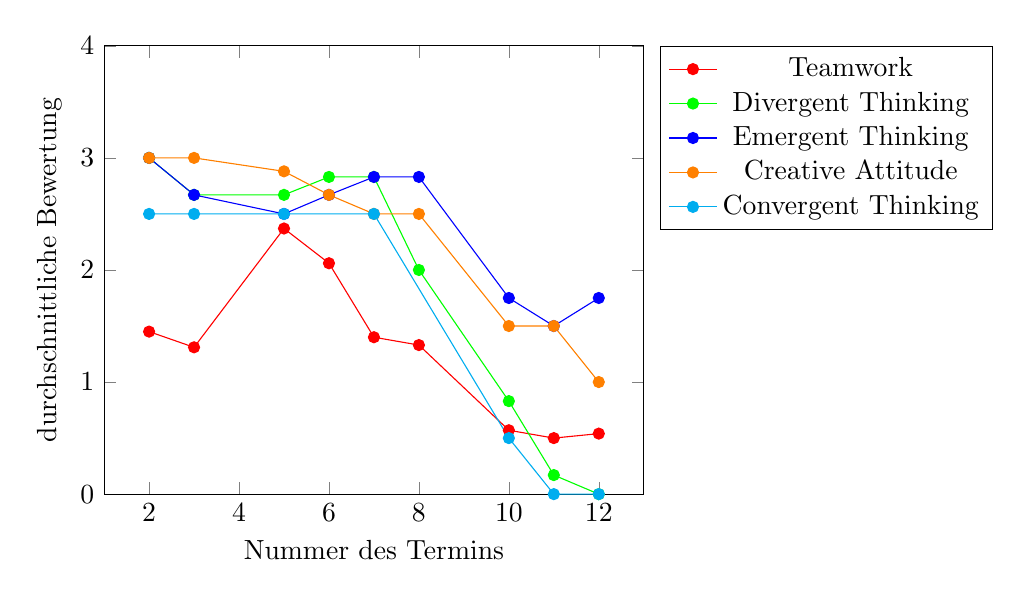
\begin{tikzpicture}
		\begin{axis}[legend pos=outer north east, ymin = 0, ymax = 4,xlabel={Nummer des Termins},ylabel={durchschnittliche Bewertung}]
			\addplot[mark=*,red]
			coordinates {
				(2,1.45)(3,1.31) (5,2.37) (6,2.06) (7,1.4) (8,1.33) (10,.57) (11,.5)(12,.54)
			};
			\addlegendentry{Teamwork}
			\addplot[mark=*, green]
			coordinates {
				(2,3)(3,2.67) (5,2.67) (6,2.83) (7,2.83) (8,2) (10,0.83) (11,0.17)(12,0)
			};
			\addlegendentry{Divergent Thinking}
			\addplot[mark=*, blue]
			coordinates {
				(2,3)(3,2.67) (5,2.5) (6,2.67) (7,2.83) (8,2.83) (10,1.75) (11,1.5)(12,1.75)
			};
			\addlegendentry{Emergent Thinking}
			\addplot[mark=*, orange]
			coordinates {
				(2,3)(3,3) (5,2.88) (6,2.67) (7,2.5) (8,2.5) (10,1.5) (11,1.5)(12,1)
			};
			\addlegendentry{Creative Attitude}
			\addplot[mark=*, cyan]
			coordinates {
				(2,2.5)(3,2.5) (5,2.5) (7,2.5) (10,0.5) (11,0)(12,0)
			};
			\addlegendentry{Convergent Thinking}
		\end{axis}
	\end{tikzpicture}
	\caption{Entwicklung von Benny}
	\label{img:bennyDevelopment}
\end{figure}
 Generell zeigte sich bei Benny in allen Bereichen ein negativer Trend. Benny startete überall mit Spitzenwerten, die deutlich über dem Durchschnitt der Werte der anderen Kinder lagen, doch im Verlauf der Kurse verschlechterten sich diese, so dass Benny in manchen Kategorien sogar mit null Punkten von den beiden Bewertern bewertet wurde. Die Gründe hierfür sind vermutlich sehr einfach zu erklären. Bennys Alter war bereits zwei Jahre über dem Alter der Mehrheit des Kurses. Dies bedeutet, dass Benny bereits einen deutlich größeres Wissen über verschiedenste Themengebiete, die in den Kursen behandelt wurden, verfügte und Fähigkeiten durch das fortgeschrittenere Alter deutlich besser ausgeprägt waren. Dazu gehörten Fähigkeiten wie das Generieren von Ideen oder Abstraktion. Die genannten Gründe könnten zu einer Unterforderung für Benny geführt haben. Dadurch ließ er sich leichter ablenken und Aufgaben, die für andere Kinder eine größere Herausforderung waren, konnte er ohne größere Schwierigkeiten lösen. Seine Entwicklung, welche in Abbildung \ref{img:bennyDevelopment} dargestellt ist, zeigt zwar eine Verschlechterung seiner Fähigkeiten, jedoch sollte dies eher als ein Verschwinden der Fähigkeiten interpretiert werden, da er seltener die geforderten Fähigkeiten einsetzte. Dies führte unter anderem auch dazu, dass seine Gruppe häufig mit Zeitproblemen zu kämpfen hatte, da sie sich viel zu sehr ablenkten. Wurden sie nach gewissen Dingen gefragt, konnten sie diese gut beantworten, selbständig verwendeten sie ihre Fähigkeiten jedoch zu selten, so dass die Qualität ihrer Bewertungen im Verlaufe des Kurses abnahm.



\subsection{Henriette}
\begin{figure}[H]
	\centering
	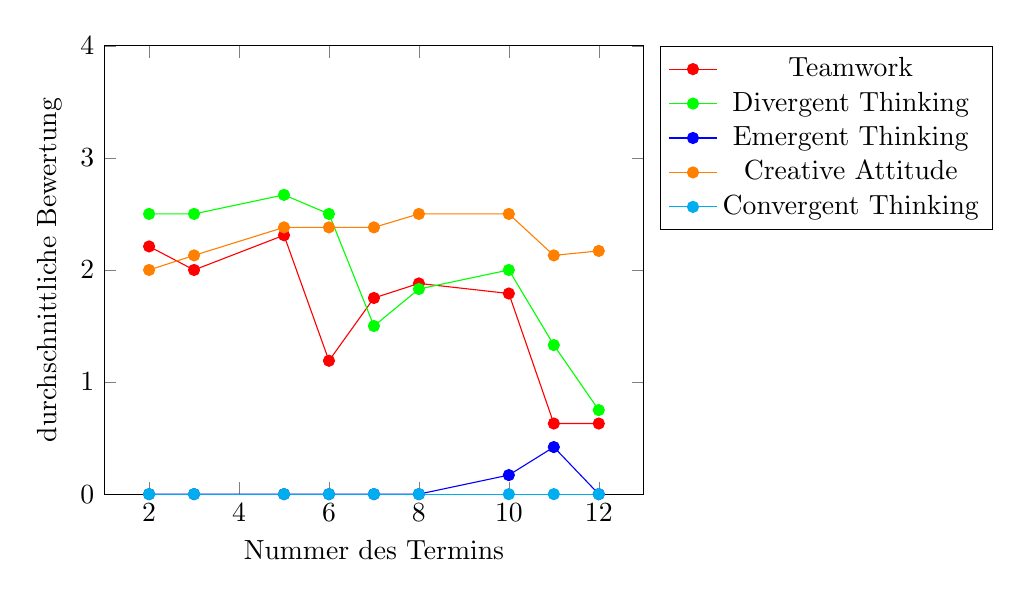
\begin{tikzpicture}
		\begin{axis}[legend pos=outer north east, ymin = 0, ymax = 4,xlabel={Nummer des Termins},ylabel={durchschnittliche Bewertung}]
			\addplot[mark=*,red]
			coordinates {
				(2,2.21)(3,2)(5,2.31)(6,1.19)(7,1.75)(8,1.88)(10,1.79)(11,0.63)(12,0.63)
			};
			\addlegendentry{Teamwork}
			\addplot[mark=*,green]
			coordinates {
				(2,2.5)(3,2.5)(5,2.67)(6,2.5)(7,1.5)(8,1.83)(10,2)(11,1.33)(12,0.75)
			};
			\addlegendentry{Divergent Thinking}
			\addplot[mark=*,blue]
			coordinates {
				(2,0)(3,0)(5,0)(6,0)(7,0)(8,0)(10,.17)(11,0.42)(12,0)
			};
			\addlegendentry{Emergent Thinking}
			\addplot[mark=*,orange]
			coordinates {
				(2,2)(3,2.13)(5,2.38)(6,2.38)(7,2.38)(8,2.5)(10,2.5)(11,2.13)(12,2.17)
			};
			\addlegendentry{Creative Attitude}
			\addplot[mark=*,cyan]
			coordinates {
				(2,0)(3,0)(5,0)(6,0)(7,0)(8,0)(10,0)(11,0)(12,0)
			};
			\addlegendentry{Convergent Thinking}
		\end{axis}
	\end{tikzpicture}
	\caption{Entwicklung von Henriette}
	\label{img:henrietteDevelopment}
\end{figure}


\subsection{Moritz}
\begin{figure}[H]
	\centering
	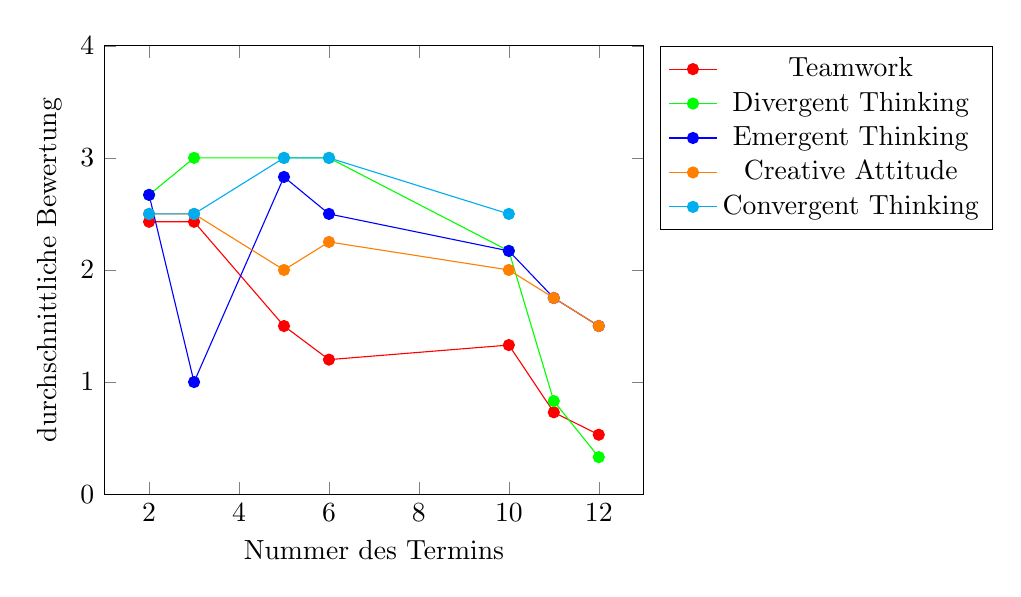
\begin{tikzpicture}
		\begin{axis}[legend pos=outer north east, ymin = 0, ymax = 4,xlabel={Nummer des Termins},ylabel={durchschnittliche Bewertung}]
			\addplot[mark=*,red]
			coordinates {
				(2,2.43)(3,2.43)(5,1.5)(6,1.2)(10,1.33)(11,.73)(12,.53)
			};
			\addlegendentry{Teamwork}
			\addplot[mark=*,green]
			coordinates {
				(2,2.67)(3,3)(5,3)(6,3)(10,2.17)(11,.83)(12,0.33)
			};
			\addlegendentry{Divergent Thinking}
			\addplot[mark=*,blue]
			coordinates {
				(2,2.67)(3,1)(5,2.83)(6,2.5)(10,2.17)(11,1.75)(12,1.5)
			};
			\addlegendentry{Emergent Thinking}
			\addplot[mark=*,orange]
			coordinates {
				(2,2.5)(3,2.5)(5,2)(6,2.25)(10,2)(11,1.75)(12,1.5)
			};
			\addlegendentry{Creative Attitude}
			\addplot[mark=*,cyan]
			coordinates {
				(2,2.5)(3,2.5)(5,3)(6,3)(10,2.5)
			};
			\addlegendentry{Convergent Thinking}
		\end{axis}
	\end{tikzpicture}
	\caption{Entwicklung von Moritz}
	\label{img:moritzDevelopment}
	
\end{figure}




\subsection{Lulu}
\begin{figure}[H]
	\centering
	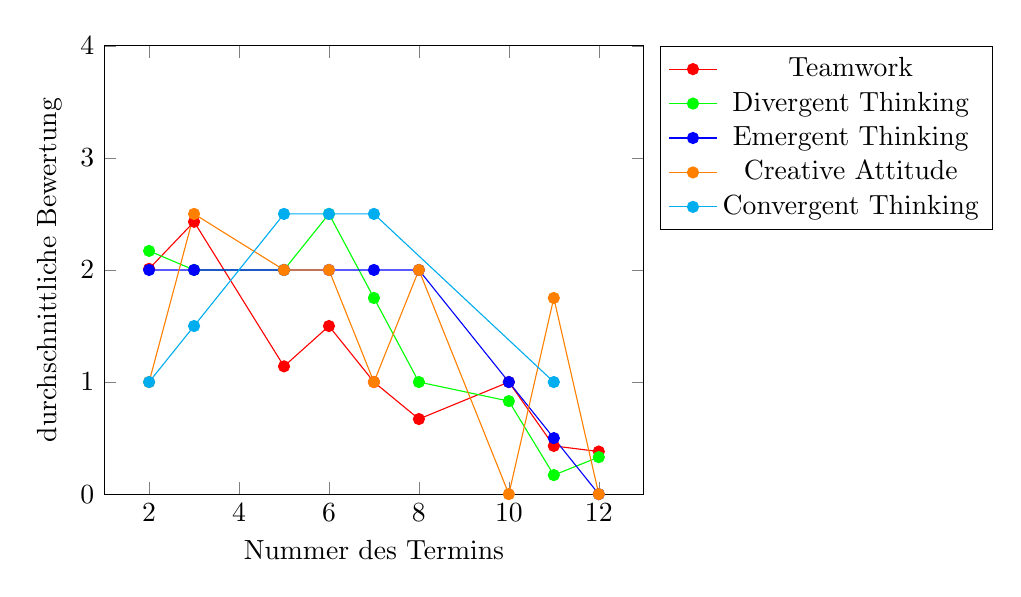
\begin{tikzpicture}
		\begin{axis}[legend pos=outer north east, ymin = 0, ymax = 4,xlabel={Nummer des Termins},ylabel={durchschnittliche Bewertung}]
			\addplot[mark=*,red]
			coordinates {
				(2,2.01)(3,2.43)(5,1.14)(6,1.5)(7,1)(8,.67)(10,1)(11,.43)(12,.38)
			};
			\addlegendentry{Teamwork}
			\addplot[mark=*,green]
			coordinates {
				(2,2.17)(3,2)(5,2)(6,2.5)(7,1.75)(8,1)(10,.83)(11,.17)(12,.33)
			};
			\addlegendentry{Divergent Thinking}
			\addplot[mark=*,blue]
			coordinates {
				(2,2)(3,2)(5,2)(6,2)(7,2)(8,2)(10,1)(11,.5)(12,0)
			};
			\addlegendentry{Emergent Thinking}
			\addplot[mark=*,orange]
			coordinates {
				(2,1)(3,2.5)(5,2)(6,2)(7,1)(8,2)(10,0)(11,1.75)(12,0)
			};
			\addlegendentry{Creative Attitude}
			\addplot[mark=*,cyan]
			coordinates {
				(2,1)(3,1.5)(5,2.5)(6,2.5)(7,2.5)(11,1)
			};
			\addlegendentry{Convergent Thinking}
		\end{axis}
	\end{tikzpicture}
	\caption{Entwicklung von Lulu}
	\label{img:luluDevelopment}	
\end{figure}





\subsection{Heinz}
\begin{figure}[H]
	\centering
	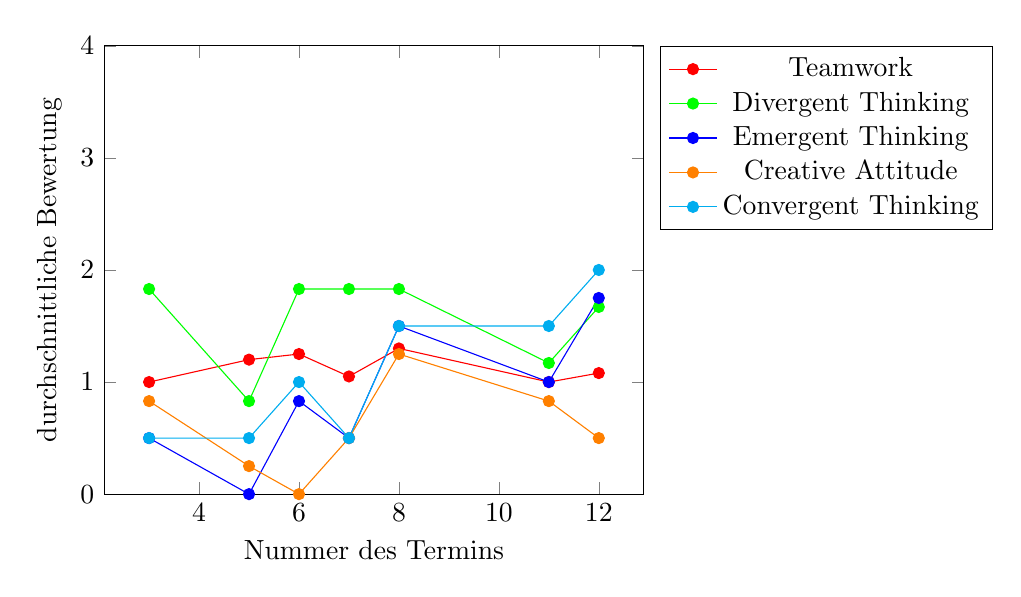
\begin{tikzpicture}
		\begin{axis}[legend pos=outer north east, ymin = 0, ymax = 4,xlabel={Nummer des Termins},ylabel={durchschnittliche Bewertung}]
			\addplot[mark=*,red]
			coordinates {
				(3,1)(5,1.2)(6,1.25)(7,1.05)(8,1.3)(11,1)(12,1.08)
			};
			\addlegendentry{Teamwork}
			\addplot[mark=*,green]
			coordinates {
				(3,1.83)(5,0.83)(6,1.83)(7,1.83)(8,1.83)(11,1.17)(12,1.67)
			};
			\addlegendentry{Divergent Thinking}
			\addplot[mark=*,blue]
			coordinates {
				(3,.5)(5,0)(6,.83)(7,.5)(8,1.5)(11,1)(12,1.75)
			};
			\addlegendentry{Emergent Thinking}
			\addplot[mark=*,orange]
			coordinates {
				(3,.83)(5,.25)(6,0)(7,.5)(8,1.25)(11,.83)(12,.5)
			};
			\addlegendentry{Creative Attitude}
			\addplot[mark=*,cyan]
			coordinates {
				(3,.5)(5,.5)(6,1)(7,.5)(8,1.5)(11,1.5)(12,2)
			};
			\addlegendentry{Convergent Thinking}
		\end{axis}
	\end{tikzpicture}
	\caption{Entwicklung von Heinz}
	\label{img:heinzDevelopment}
	
\end{figure}


\section{Persönlichkeitstypen und Entwicklung} \label{sec:personalityAndDevelopment}
\subsection{Teamwork}
\begin{figure}[H]
	\centering
	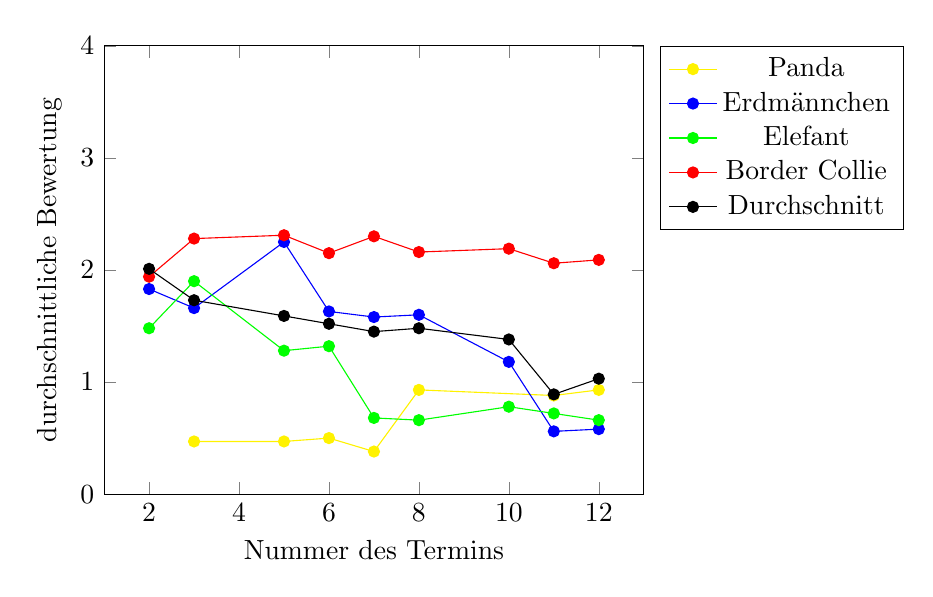
\begin{tikzpicture}
		\begin{axis}[legend pos=outer north east, ymin = 0, ymax = 4,xlabel={Nummer des Termins},ylabel={durchschnittliche Bewertung}]
			\addplot[mark=*,yellow]
			coordinates {
				(3,.47) (5,.47) (6,.5) (7,.38) (8,0.93) (11,.88) (12,.93)
			};
			\addlegendentry{Panda}
			\addplot[mark=*,blue]
			coordinates {
				(2,1.83)(3,1.66)(5,2.25)(6,1.63)(7,1.58)(8,1.6)(10,1.18)(11,.56)(12,.58)
			};
			\addlegendentry{Erdmännchen}
			\addplot[mark=*,green]
			coordinates {
				(2,1.48)(3,1.9)(5,1.28)(6,1.32)(7,0.68)(8,0.66)(10,.78)(11,.72)(12,.66)
			};
			\addlegendentry{Elefant}
			\addplot[mark=*,red]
			coordinates {
				(2,1.94)(3,2.28)(5,2.31)(6,2.15)(7,2.3)(8,2.16)(10,2.19)(11,2.06)(12,2.09)
			};
			\addlegendentry{Border Collie}
			\addplot[mark=*, black]
			coordinates{
				(2,2.01)(3,1.73)(5,1.59)(6,1.52)(7,1.45)(8,1.48)(10,1.38)(11,0.89)(12,1.03)
			};
			\addlegendentry{Durchschnitt}
		\end{axis}
	\end{tikzpicture}
	\caption{Entwicklung der Teamarbeitsfähigkeit}
	\label{img:teamDevelopment}
\end{figure}
Abbildung \ref{img:teamDevelopment} zeigt, wie sich das Verhalten der Kinder im Verlaufe der Termine entwickelt hat. Dazu wurde der Durchschnitt der Kinder eines Persönlichkeitstyps im Diagramm eingetragen. An Terminen, an denen ein Kind aufgrund Krankheit oder anderen Gründen nicht teilnehmen konnten, hatten keine Auswirkungen auf den Durchschnitt an diesem Termin, an diesen wurde dann der Durchschnitt aus den verbleibenden Kindern dieses Typs genommen.\\
Zuerst die generelle Entwicklung der Kinder der Studie. Die Fähigkeit, im Team zu arbeiten, nimmt im Verlauf des Kurses ab. Nur hin und wieder verbessert sich die Bewertungen der Kinder, jedoch nur in sehr geringem Ausmaß.\\
Da Sara das einzige Kind der Kategorie Panda ist, zeigt die obenstehende Abbildung, dass sich Pandas im Umgang mit Technologie im Rahmen der Studie ihre Teamfähigkeit verbessert haben. Da aber sie der einzige Panda der Studie ist, kann hier nicht generalisiert werden und auf andere Pandas geschlossen werden. Im Vergleich zu den anderen Kindern zeigt der Panda zwar eine Verbesserung, aber selbst das Maximum ihrer Teamfähigkeit übertrifft die Minima der anderen Kinder nur knapp und liegt durchgehend unter dem Durchschnitt. Ein Grund für das schlechte Abschneiden im Vergleich zu den Kindern kann ihre Schüchternheit sein, die während den Terminen oft an den Tag trat. Dadurch hatte sie Schwierigkeiten, sich im Team zu erweisen.\\
Die Kinder der Typen Border Collie zeigten keine Entwicklung in ihrer Teamfähigkeit, dafür ist diese jedoch im Verlaufe des Kurses konstant. An vielen Tagen haben diese Kinder eine der höchsten durchschnittlichen Bewertungen, wie aus Abb. \ref{img:teamDevelopment} hervor geht. Insgesamt ist ihre Teamfähigkeit innerhalb der Studie an der \acrshort{dhbw} Karlsruhe als überdurchschnittlich zu bewerten. Ein Grund dafür ist unter anderem die Konstanz der beiden Kinder. Bei den Teamaufgaben arbeiteten die beiden oft zusammen, die Angehörigkeit des gleichen Typs kann ein Grund für die durchgehende Konstanz ihrer Teamfähigkeit ist.\\
Die Kinder, die in ihrem Persönlichkeitstest als Ergebnis Elefant bekommen haben, verschlechterten sich in ihrer Teamfähigkeit deutlich. In den meisten Fällen ist ihre durchschnittliche Bewertung auch unterhalb des Durchschnitts der gesamten Gruppe. Grund hierfür wird vermutlich Unterforderung sein. Wie die Abbildungen \ref{img:auswertung_typus} und \ref{img:auswertung_typus_ctt} zeigen, erreichen die Kinder Höchstwerte in den einzelnen Kategorien, selbst bei dem schwierigen Test erzielten die Kinder sehr gute Ergebnisse. Für diese Kinder wäre es möglich, auch mit der nächsten Stufe der programmierbaren Roboter von Lego zu arbeiten. Die Unterforderung kann auch alterstechnisch bedingt sein. Moritz war während der Kurse bereits in der 4. Klasse und damit zwei Klassenstufen über den anderen Kindern.\\
Ebenso eine Verschlechterung zeigten die Kinder des Persönlichkeitstyps Erdmännchen. Anders als die Elefanten lag ihr Durchschnitt öfters über dem Durchschnitt aller Kinder und auch meist höher als der der Elefanten. Auch hier kann wieder als möglicher Grund für die Verschlechterung die Unterforderung der Kinder genannt werden. Erdmännchen erzielten in den Tests gute Ergebnisse und auch Benny besuchte bereits die 4. Klasse, weshalb sein Wissen und seine geistigen Fähigkeiten auf einem höheren Niveau lagen. 


\subsection{Divergentes Denken}
\begin{figure}[H]
	\centering
	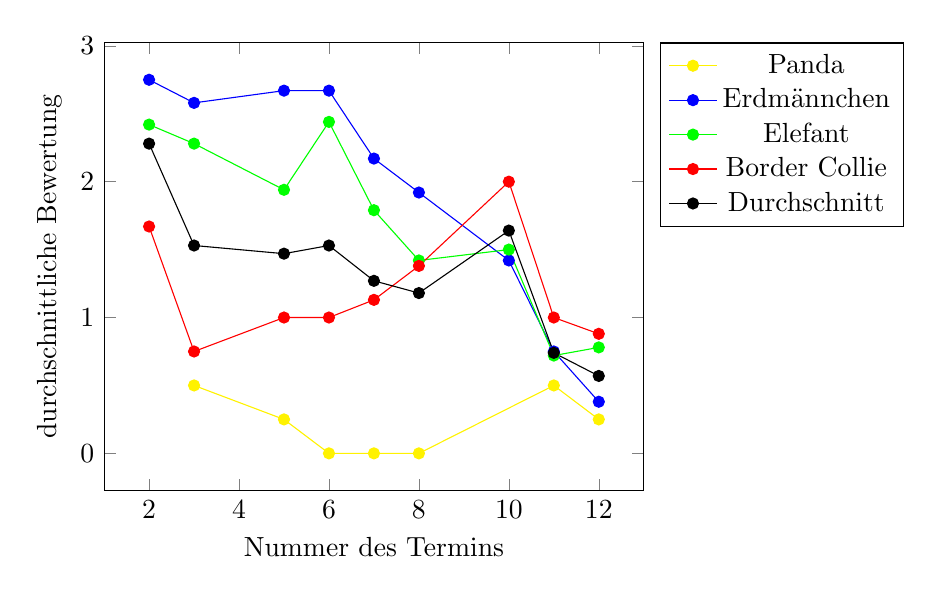
\begin{tikzpicture}
		\begin{axis}[legend pos=outer north east,xlabel={Nummer des Termins},ylabel={durchschnittliche Bewertung}]
			\addplot[mark=*,yellow]
			coordinates {
				(3,.5) (5,.25) (6,0) (7,0) (8,0) (11,.5) (12,.25)
			};
			\addlegendentry{Panda}
			\addplot[mark=*,blue]
			coordinates {
				(2,2.75)(3,2.58)(5,2.67)(6,2.67)(7,2.17)(8,1.92)(10,1.42)(11,.75)(12,.38)
			};
			\addlegendentry{Erdmännchen}
			\addplot[mark=*,green]
			coordinates {
				(2,2.42)(3,2.28)(5,1.94)(6,2.44)(7,1.79)(8,1.42)(10,1.5)(11,.72)(12,.78)
			};
			\addlegendentry{Elefant}
			\addplot[mark=*,red]
			coordinates {
				(2,1.67)(3,.75)(5,1)(6,1)(7,1.13)(8,1.38)(10,2)(11,1)(12,.88)
			};
			\addlegendentry{Border Collie}
			\addplot[mark=*,black]%Germany
			coordinates {
				(2,2.28) (3,1.53) (5,1.47) (6,1.53) (7,1.27) (8,1.18) (10,1.64)(11,.74) (12,.57)
			};
			\addlegendentry{Durchschnitt}
			
		\end{axis}
	\end{tikzpicture}
	\caption{Entwicklung des divergenten Denkens}
\end{figure}	
Im Bereich des divergenten Denkens schneiden die Erdmännchen zu Beginn am besten und die Pandas am schlechtesten ab. Im Verlauf ist bei den Erdmännchen und den Elefanten ein starker Abwärtstrend erkennbar. Am Ende liegen alle Persönlichkeitstypen bei Werten unter 1, wobei die Border Collies noch am besten abschneiden.

\subsection{Emergentes Denken}
\begin{figure}[H]
	\centering
	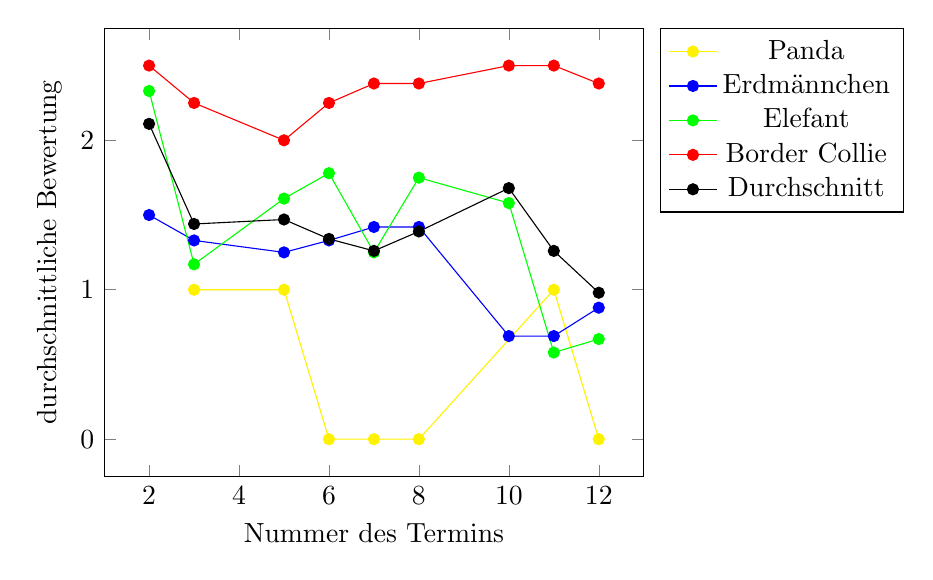
\begin{tikzpicture}
		\begin{axis}[legend pos=outer north east,xlabel={Nummer des Termins},ylabel={durchschnittliche Bewertung}]
			\addplot[mark=*,yellow]
			coordinates {
				(3,1) (5,1) (6,0) (7,0) (8,0) (11,1) (12,0)
			};
			\addlegendentry{Panda}
			\addplot[mark=*,blue]
			coordinates {
				(2,1.5)(3,1.33)(5,1.25)(6,1.33)(7,1.42)(8,1.42)(10,.69)(11,.69)(12,.88)
			};
			\addlegendentry{Erdmännchen}
			\addplot[mark=*,green]
			coordinates {
				(2,2.33)(3,1.17)(5,1.61)(6,1.78)(7,1.25)(8,1.75)(10,1.58)(11,.58)(12,.67)
			};
			\addlegendentry{Elefant}
			\addplot[mark=*,red]
			coordinates {
				(2,2.5)(3,2.25)(5,2)(6,2.25)(7,2.38)(8,2.38)(10,2.5)(11,2.5)(12,2.38)
			};
			\addlegendentry{Border Collie}
			\addplot[mark=*,black]%Germany
			coordinates {
				(2,2.11) (3,1.44) (5,1.47) (6,1.34) (7,1.26) (8,1.39) (10,1.68)(11,1.26) (12,.98)
			};
			\addlegendentry{Durchschnitt}
			
		\end{axis}
	\end{tikzpicture}
	\caption{Entwicklung des emergenten Denkens}
\end{figure}	
Betrachtet man das emergente Denken fällt auf,  dass die Border Collies mit Werten über 2 deutlich über den anderen Persönlichkeitstypen liegen. Die Pandas schneiden hier am schlechtesten ab und kommen nicht über einen Wert von 1 hinaus. Auch die Elefanten, die zu Beginn Werte nahe der Border Collies erzielen, liegen gegen Ende bei einem Wert unter 1. Im Durchschnitt lässt sich auch ein negativer Trend beobachten, hier liegt der Unterschied zwischen dem Maximum zu Beginn und dem Minimum gegen Ende bei knapp 1.25.


\subsection{Kreative Haltung}
\begin{figure}[H]
	\centering
	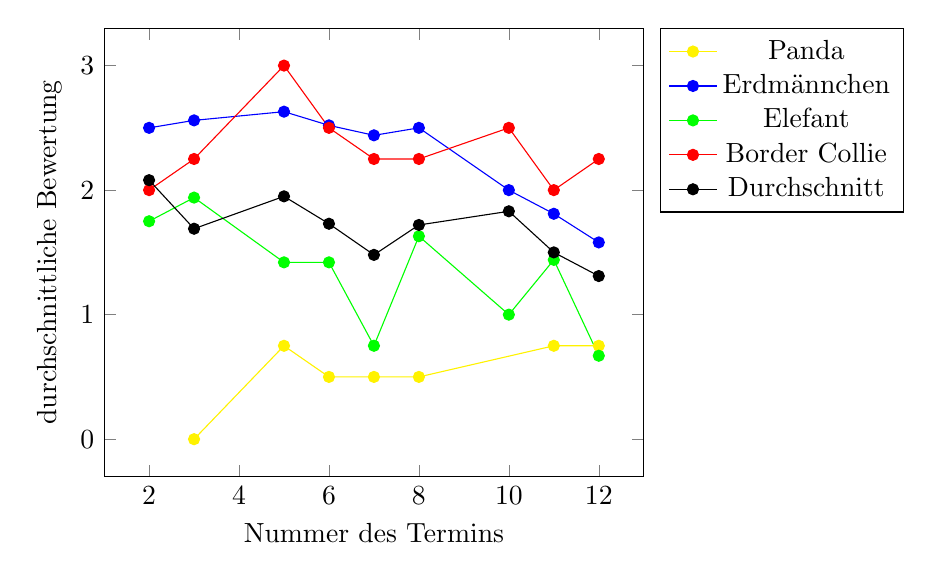
\begin{tikzpicture}
		\begin{axis}[legend pos=outer north east,xlabel={Nummer des Termins},ylabel={durchschnittliche Bewertung}]
			\addplot[mark=*,yellow]
			coordinates {
				(3,0) (5,.75) (6,.5) (7,.5) (8,.5) (11,.75) (12,.75)
			};
			\addlegendentry{Panda}
			\addplot[mark=*,blue]
			coordinates {
				(2,2.5)(3,2.56)(5,2.63)(6,2.52)(7,2.44)(8,2.5)(10,2)(11,1.81)(12,1.58)
			};
			\addlegendentry{Erdmännchen}
			\addplot[mark=*,green]
			coordinates {
				(2,1.75)(3,1.94)(5,1.42)(6,1.42)(7,0.75)(8,1.63)(10,1)(11,1.44)(12,.67)
			};
			\addlegendentry{Elefant}
			\addplot[mark=*,red]
			coordinates {
				(2,2)(3,2.25)(5,3)(6,2.5)(7,2.25)(8,2.25)(10,2.5)(11,2)(12,2.25)
			};
			\addlegendentry{Border Collie}
			\addplot[mark=*,black]%Germany
			coordinates {
				(2,2.08) (3,1.69) (5,1.95) (6,1.73) (7,1.48) (8,1.72) (10,1.83)(11,1.5) (12,1.31)
			};
			\addlegendentry{Durchschnitt}
			
		\end{axis}
	\end{tikzpicture}
	\caption{Entwicklung der kreativen Haltung}
\end{figure}	
Im Bereich der kreativen Haltung schneiden die Pandas erneut am schlechtesten ab, sie pendeln sich nach einer leichten Verbesserung zu Beginn bei einem Wert um die 0.75 ein. Die Erdmännchen starten mit einem Wert von 2.5 am besten fallen aber im Verlauf um 1 auf ungefähr 1.5 ab. Die Erdmännchen starten bei 2 und pendeln sich mit leichten Ausreißern auf 2.25 ein. Die Elefanten bewegen sich im Mittelfeld und liegen leicht unter dem Durchschnitt, welcher im Bereich von 1.5 und 2 liegt. Allgemein ist in diesem Bereich bei keiner Gruppe eine positive Veränderung zu erkennen, ausgenommen der Pandas.	
	
\subsection{Konvergentes Denken}
\begin{figure}[H]
	\centering
	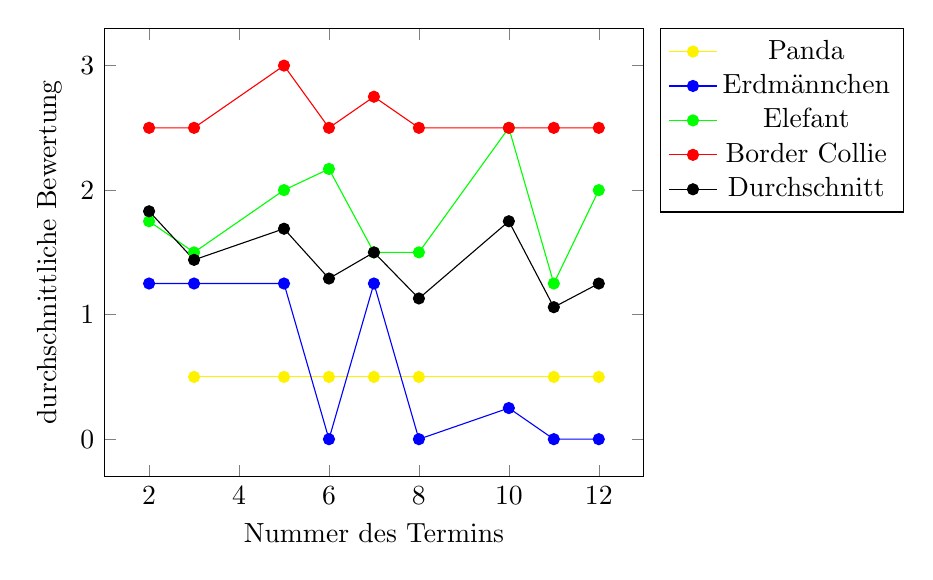
\begin{tikzpicture}
		\begin{axis}[legend pos=outer north east,xlabel={Nummer des Termins},ylabel={durchschnittliche Bewertung}]
			\addplot[mark=*,yellow]
			coordinates {
				(3,.5) (5,.5) (6,.5) (7,.5) (8,.5) (11,.5) (12,.5)
			};
			\addlegendentry{Panda}
			\addplot[mark=*,blue]
			coordinates {
				(2,1.25)(3,1.25)(5,1.25)(6,0)(7,1.25)(8,0)(10,.25)(11,0)(12,0)
			};
			\addlegendentry{Erdmännchen}
			\addplot[mark=*,green]
			coordinates {
				(2,1.75)(3,1.5)(5,2)(6,2.17)(7,1.5)(8,1.5)(10,2.5)(11,1.25)(12,2)
			};
			\addlegendentry{Elefant}
			\addplot[mark=*,red]
			coordinates {
				(2,2.5)(3,2.5)(5,3)(6,2.5)(7,2.75)(8,2.5)(10,2.5)(11,2.5)(12,2.5)
			};
			\addlegendentry{Border Collie}
			\addplot[mark=*,black]%Germany
			coordinates {
				(2,1.83) (3,1.44) (5,1.69) (6,1.29) (7,1.5) (8,1.13) (10,1.75)(11,1.06) (12,1.25)
			};
			\addlegendentry{Durchschnitt}
			
		\end{axis}
	\end{tikzpicture}
	\caption{Entwicklung des konvergenten Denkens}
\end{figure}	
Beim konvergenten Denken fällt auf, dass die Border Collies im kompletten Zeitablauf über allen anderen Persönlichkeitstypen liegen, sie halten sich konstant bei Werten um die 2.5. Die Elefanten bewegen sich nahe am Durchschnitt und erreichen im Maximum sogar das Niveau der Border Collies. Die Erdmännchen liegen im kompletten Verlauf unter dem Durchschnitt und haben einen negativen Abfall verglichen zum Anfangsniveau. Die Pandas haben einen konstanten Verlauf von 0.5. Insgesamt lässt sich hier sagen, dass es große Unterschiede zwischen den einzelnen Gruppen gibt und wenige Schnittpunkte unter den Gruppen gibt
\section{Herkunft und Entwicklung}
Da wie bereits erwähnt die Daten der Parallelveranstaltung in Ägypten keine Vergleichsdaten zu den Persönlichkeitstests und den Computational Thinking Tests liefern, ist nur ein kultureller Vergleich beider Gruppen möglich. Deshalb werden im folgenden Abschnitt die beiden Studien in den fünf Bereichen miteinander verglichen.
\subsection{Teamwork}
\begin{figure}[H]
	\centering
	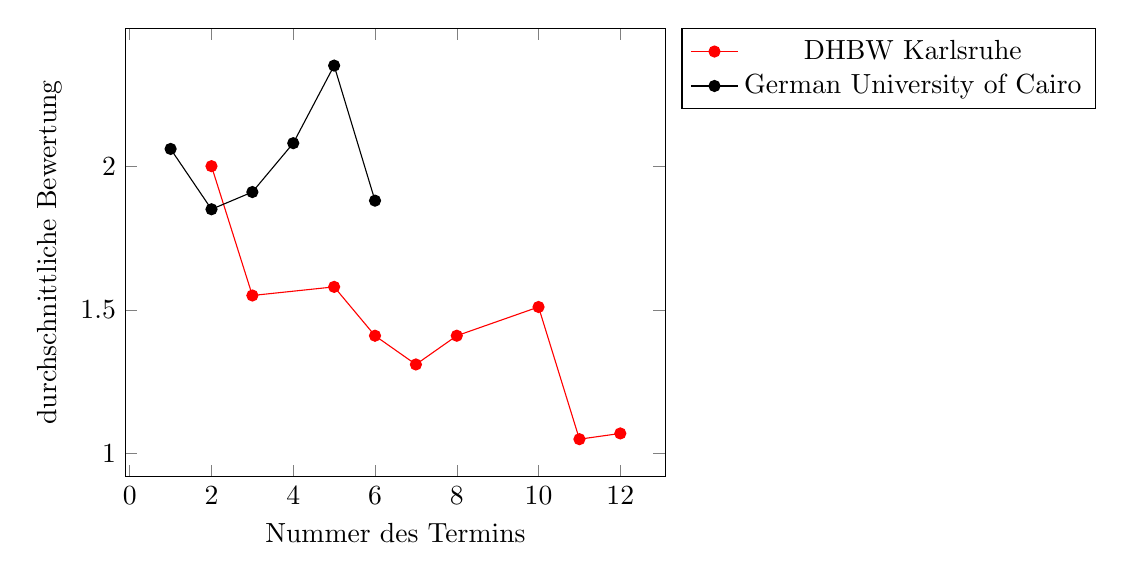
\begin{tikzpicture}
		\begin{axis}[legend pos=outer north east,xlabel={Nummer des Termins},ylabel={durchschnittliche Bewertung}]
			\addplot[mark=*,red]%Germany
			coordinates{
				(2,2)(3,1.55)(5,1.58)(6,1.41)(7,1.31)(8,1.41)(10,1.51)(11,1.05)(12,1.07)
			};
			\addlegendentry{DHBW Karlsruhe}
			\addplot[mark=*,black]
			coordinates {
				(1,2.06)(2,1.85)(3,1.91)(4,2.08)(5,2.35)(6,1.88)
			};
			\addlegendentry{German University of Cairo}
			
		\end{axis}
	\end{tikzpicture}
	\caption{Entwicklung des konvergenten Denkens}
\end{figure}
Vergleicht man das Teamwork von Deutschland und Kairo, sieht man bei beiden Gruppen einen ähnliches Anfangsniveau von knapp über 2. Während in Kairo das Teamwork dann ansteigt und erst zum letzten Termin wieder knapp unter den Anfangstrend fällt, sinkt es in Karlsruhe immer weiter bis auf knapp 1 ab. Beim Vergleich der beiden Gruppen muss jedoch auch die unterschiedliche Gruppengröße und die Anzahl der Termine berücksichtigt werden.
\subsection{Divergentes Denken}
\begin{figure}[H]
	\centering
	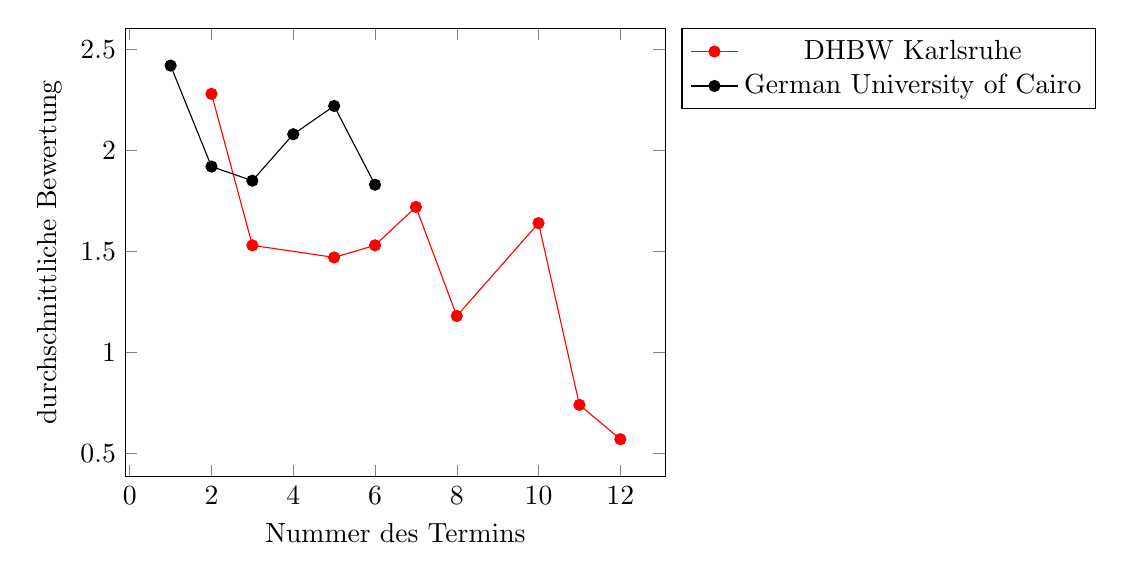
\begin{tikzpicture}
		\begin{axis}[legend pos=outer north east,xlabel={Nummer des Termins},ylabel={durchschnittliche Bewertung}]
			\addplot[mark=*,red]%Germany
			coordinates {
				(2,2.28) (3,1.53) (5,1.47) (6,1.53) (7,1.72) (8,1.18) (10,1.64)(11,.74) (12,.57)
			};
			\addlegendentry{DHBW Karlsruhe}
			\addplot[mark=*,black]
			coordinates {
				(1,2.42)(2,1.92)(3,1.85)(4,2.08)(5,2.22)(6,1.83)
			};
			\addlegendentry{German University of Cairo}
			
		\end{axis}
	\end{tikzpicture}
	\caption[Vergleich Entwicklung Teamfähigkeit beider Veranstaltungen]{Vergleich der Entwicklung der Teamfähigkeit beider Veranstaltungen}
\end{figure}
Auch hier sieht man bei beiden Gruppen ein ähnliches Ausgangsniveau, jedoch fällt auch hier das divergente Denken im verlauf ab. Bei der deutschen Gruppe wird auch hier fast ein Wert nahe 0 erzielt. 
\subsection{Emergentes Denken}
\begin{figure}[H]
	\centering
	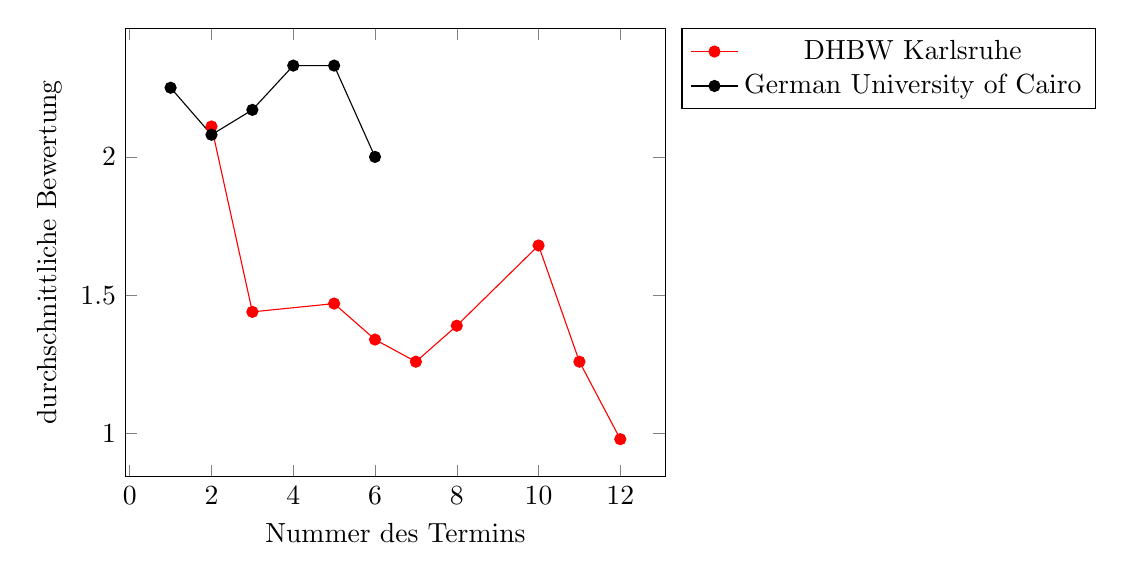
\begin{tikzpicture}
		\begin{axis}[legend pos=outer north east,xlabel={Nummer des Termins},ylabel={durchschnittliche Bewertung}]
			\addplot[mark=*,red]%Germany
			coordinates {
				(2,2.11) (3,1.44) (5,1.47) (6,1.34) (7,1.26) (8,1.39) (10,1.68)(11,1.26) (12,.98)
			};
			\addlegendentry{DHBW Karlsruhe}
			\addplot[mark=*,black]
			coordinates {
				(1,2.25)(2,2.08)(3,2.17)(4,2.33)(5,2.33)(6,2)
			};
			\addlegendentry{German University of Cairo}
			
		\end{axis}
	\end{tikzpicture}
	\caption[Vergleich Entwicklung emergentes Denken beider Veranstaltungen]{Vergleich der Entwicklung des emergenten Denkens beider Veranstaltungen}
\end{figure}
Ebenfalls beim emergenten Denken starten beide Gruppen bei einem ähnlichen Level von um die 2. die Zeitverlauf fallen wieder beide Gruppen deutlich ab, Deutschland liegt auch heir unter Ägypten.
\subsection{Kreative Haltung}
\begin{figure}[H]
	\centering
	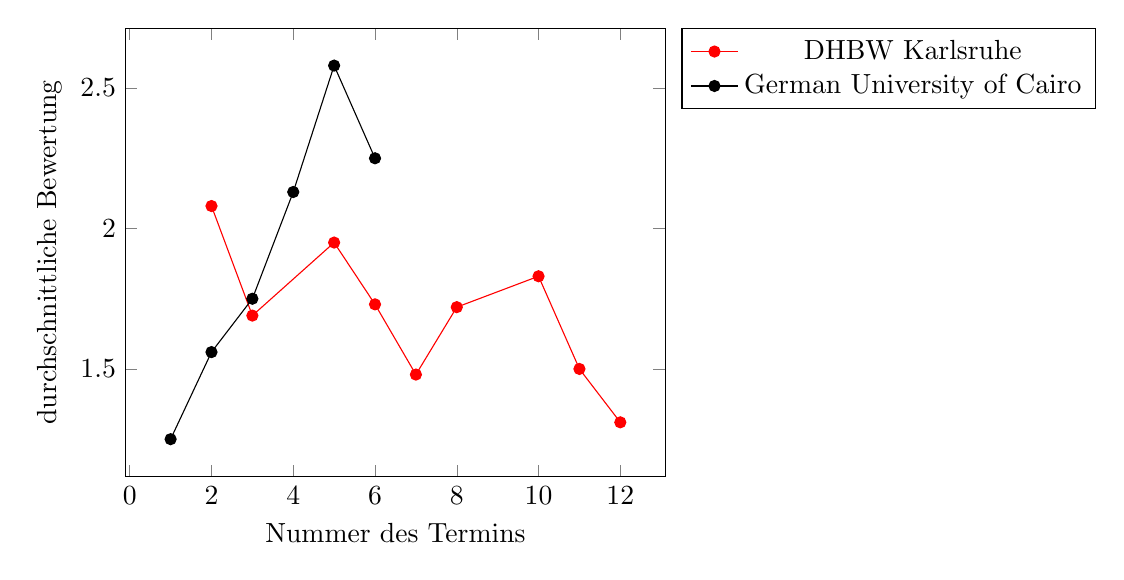
\begin{tikzpicture}
		\begin{axis}[legend pos=outer north east,xlabel={Nummer des Termins},ylabel={durchschnittliche Bewertung}]
			\addplot[mark=*,red]%Germany
			coordinates {
				(2,2.08) (3,1.69) (5,1.95) (6,1.73) (7,1.48) (8,1.72) (10,1.83)(11,1.5) (12,1.31)
			};
			\addlegendentry{DHBW Karlsruhe}
			\addplot[mark=*,black]
			coordinates {
				(1,1.25)(2,1.56)(3,1.75)(4,2.13)(5,2.58)(6,2.25)
			};
			\addlegendentry{German University of Cairo}
			
		\end{axis}
	\end{tikzpicture}
	\caption[Vergleich Entwicklung kreative Haltung beider Veranstaltungen]{Vergleich der Entwicklung der kreativen Haltung beider Veranstaltungen}
\end{figure}
Ebenfalls beim emergenten Denken starten beide Gruppen bei einem ähnlichen Level von um die 2. die Zeitverlauf fallen wieder beide Gruppen deutlich ab, Deutschland liegt auch heir unter Ägypten.
\subsection{Konvergentes Denken}
\begin{figure}[H]
	\centering
	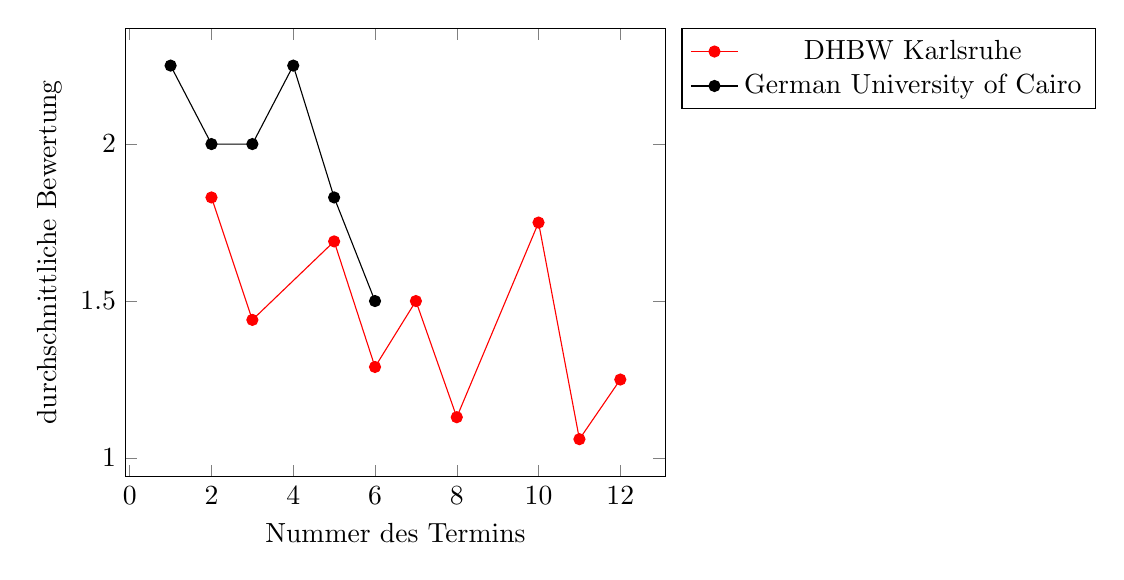
\begin{tikzpicture}
		\begin{axis}[legend pos=outer north east,xlabel={Nummer des Termins},ylabel={durchschnittliche Bewertung}]
			\addplot[mark=*,red]%Germany
			coordinates {
				(2,1.83) (3,1.44) (5,1.69) (6,1.29) (7,1.5) (8,1.13) (10,1.75)(11,1.06) (12,1.25)
			};
			\addlegendentry{DHBW Karlsruhe}
			\addplot[mark=*,black]
			coordinates {
				(1,2.25)(2,2)(3,2)(4,2.25)(5,1.83)(6,1.5)
			};
			\addlegendentry{German University of Cairo}
			
		\end{axis}
	\end{tikzpicture}
	\caption[Vergleich Entwicklung konvergentes Denken beider Veranstaltungen]{Vergleich der Entwicklung des konvergenten Denkens beider Veranstaltungen}
\end{figure}
Im Bereich des konvergenten Denkens sieht man einen guten Start bei der ägyptischen Gruppe jedoch fällt diese im verlauf fast um 1. Die deutsche Gruppe hat einige Ausschläge nach oben und ist im Durchschnitt bei einem Wert um die 1.5.
\section{Computational Thinking Test}
	In dem folgenden Abschnitt wird die Auswertung der Ergebnisse des \acrshort{bctt}, welcher zu Beginn der Studie durchgeführt wurde, sowie die des \acrshort{cctt}, welcher nach Abschluss aller Termine von den Kindern bearbeitet wurde. Die Ergebnisse der beiden Tests befinden sich im Kapitel \ref{sec:ErgebnisseCTT}.
	\subsection{BCTt}
	In Kapitel \ref{sec:ct} wurde aufgeführt, welche Ergebnisse bei einer Durchführung des \acrshort{bctt} bei einer Stichprobe von 299 Schülern und Schülerinnen auftreten. Anhand dieser Daten kann nun die Gruppe der Kinder, die an dieser Studie an der \acrshort{dhbw} Karlsruhe teilnahmen, in ihrem informatischen Denken eingeordnet werden. Dazu werden die Daten der Kinder aus Tabelle \ref{tab:data} in der untenstehenden Tabelle noch einmal aufbereitet, so dass ein guter Vergleich gezogen werden kann. Generell ist zu beachten, dass die Stichprobe, die von \citeauthor{bcct} aufgeführt wurde, eine deutlich höhere Anzahl an Teilnehmern hat als die Anzahl, die in dieser Studienarbeit zur Verfügung stand. Dadurch kann nur beurteilt werden, ob die Kinder dieser Studie dem Durchschnitt entsprachen oder über- bzw. unterdurchschnittlich abschnitten.
	\begin{table}[H]
		\centering
		\begin{tabular}{|l|l|l|l|}
			\hline
			\rowcolor[HTML]{C0C0C0} 
			\textbf{Klassenstufe} & \textbf{Anzahl} & \textbf{Durchschnitt} & \textbf{Std. Abweichung} \\ \hline
			2                     & 6               & 19.5                  & 5,188                    \\ \hline
			3                     & 2               & 24                    & 1                        \\ \hline
		\end{tabular}
	\label{tab:statisticAufbereitung}
	\caption{Statistische Aufbereitung der Werte der Tabelle \ref{tab:data}}
	\end{table}

	Für die Altersgruppe der Kinder, die sich während des Tests in der dritten Klassenstufe befanden, existieren seitens der Autoren des \acrshort{bctt} keine Vergleichsdaten. Die Kinder, die die dritte Stufe besuchten, übertrafen im Vergleich zu den Daten aus Tabelle \ref{tab:statisticsBCTT}. Diese Kinder schnitten im Durchschnitt besser ab und die Standardabweichung lag auch deutlich unter den von \citeauthor{bcct} angegebenen Daten. Die Stichprobe, die von den Autoren dieser Studienarbeit durchgeführt wurde, ist jedoch nicht sehr groß, weshalb die Aussagekraft über das Abschneiden der Kinder nicht sehr hoch ist.\\
	Anders sieht es bei den Kindern der Klassenstufe Zwei aus. Wie aus der obenstehenden Tabelle zu entnehmen ist, lag der Durchschnitt, den die Kinder beim Bearbeiten des \acrlong{bctt} erzielten, zwar ebenfalls über dem Durchschnitt aus Tabelle \ref{tab:statisticsBCTT}, jedoch ist die Standardabweichung, die für diese Gruppe ermittelt wurde, doppelt so hoch als die Vergleichsdaten der Kinder aus Spanien. Wie aus der Tabelle \ref{tab:data} erkennbar ist, lag die Streuung der Ergebnisse der Kinder, die die Klassenstufe Zwei besuchten, in einem Bereich von 10 Punkten bis hin zur maximal erreichbaren Punktzahl von 25 Punkten.   
	\subsection{CCTt}
	Der \acrshort{cctt} fiel im Vergleich zum \acrshort{bctt} wie erwartet schlechter aus. Wenig überraschend dagegen ist das Abschneiden der Elefanten und auch das der Erdmännchen, da diese bereits im \acrshort{bctt} sehr gut abgeschnitten hatten. Ein großes Problem der Kinder war die Zeit. Das wird anhand der Punkte, die die Kinder in den einzelnen Kategorien erreicht haben, ersichtlich, da Kategorien, die weiter hinten angesiedelt waren, aufgrund der Zeit nicht bearbeitet wurden. Auffallend sind daher die Ergebnisse des Persönlichkeitstyps Panda, da dieser im \acrshort{bctt} schlechter abgeschnitten hatte. Da alle anderen Gruppen in den Typen weiter rechts auf der X-Achse weniger Punkte sammelten und auch bei Sara kein zufälliges bzw. unsortiertes Lösen der Aufgaben beobachtet werden konnte, gibt es hierfür einen anderen Grund. Beim Korrigieren des \acrshort{cctt} ist aufgefallen, dass weiter hinten Sara vermutlich aus Zeitgründen immer die gleiche Antwort angekreuzt hat. Dadurch hatte sie viel Glück und die Antworten waren sogar teilweise richtig, jedoch verfälschte das das Ergebnis. Also wurde um Glücksantworten zu filtern für falsche Fragen ein Minuspunkt berechnet, für nicht beantwortete Fragen kein Punkt. So kann überprüft werden, ob die Kinder wirklich die Antworten wussten oder eben Glückstreffer dabei waren. Dabei ergab sich nach Abzug der falschen Punkte die untenstehenden Werte.
	
	
	\pgfplotstableread[row sep=\\,col sep=&]{
		Name &Ohne Abzug &Mit Abzug \\
		Henriette     & 4  & 1 \\
		Moritz     & 16 & 15 \\
		Heinz    & 0 & 0\\
		Benny   & 11 & 11\\
		Lulu   & 6  & 4\\
		Mario      & 3 & -5\\
		Sara &6 & -6\\
		Jonas&3 & -2\\
	}\mydata

	\begin{figure}[H]
		\begin{tikzpicture}
			\begin{axis}[ ybar,
				bar width=.5cm,
				width=\textwidth,
				height=.5\textwidth,
				legend style={at={(0.5,1)},
					anchor=north,legend columns=-1},
				symbolic x coords={Henriette, Moritz, Heinz, Benny, Lulu, Mario, Sara, Jonas},
				xtick=data,
				nodes near coords,
				nodes near coords align={vertical},
				ymin=-10,ymax=20,
				ylabel={Anzahl erreichter Punkte}, xlabel = {Name des Kindes}]
				\addplot table[x=Name,y=Ohne Abzug]{\mydata};
				\addplot table[x=Name,y=Mit Abzug]{\mydata};
				\addlegendentry{Ohne Abzug}
				\addlegendentry{Mit Abzug}
			\end{axis}
		\end{tikzpicture}
		\caption[Änderungen Punktzahlen nach Abzug]{Änderungen der Punktzahlen nach Abzug der falschen Antworten}
		\label{img:wrongAnswerCorrection}
	\end{figure}

	Auffallend ist, wie bereits vermutet, das Ergebnis von Sara. Statt voher insgesamt sechs korrekt beantworteten Fragen hatte sie nun ein Ergebnis von -6, also zwölf falsch beantwortete Fragen. Natürlich kann hier angemerkt werden, dass die Kinder nicht wussten, dass wir für falsche Fragen Punkte abziehen, ihre Anweisungen waren lediglich: \glqq Es ist nicht wichtig, dass du alle Fragen beantwortest\grqq. Deshalb könnte dies anders ausfallen, sollten die Kinder vorher darüber informiert werden. Bei dem Großteil der Kinder zeigte sich jedoch, dass die Fragen, die sie beantwortet hatten, korrekt waren und Fragen, die sie nicht beantworten konnten, übersprungen wurden. Die Abzüge waren meist nur sehr gering. Lediglich die 12-Punkte-Differenz bei Sara zeigt, dass die Ergebnisse aus \ref{img:auswertung_typus_ctt} verfälscht sind und man daraus nicht schließen kann, dass sie in diesen Bereichen besser ist als die anderen Kinder.\\
	Ebenso ist auch das Ergebnis von Mario. Auch er verlor einen Großteil seiner Punkte durch den Abzug falscher Antworten. Er hatte den Test nach nicht einmal sieben Minuten beendet und einige Aufgaben übersprungen, bei denen er keine Antwort wusste. Statt die 13 Minuten, die er noch hatte, zu nutzen und seine Antworten zu überprüfen, gab er ab und schnitt dementsprechend schlecht ab. Hier spielte also weniger die Zeit eine Rolle, als das Wissen bzw. die Fähigkeit, das Computational Thinking anzuwenden.\\
	Aufgrund der nicht zufälligen Bearbeitung kann für weiter hinten angesiedelte Typen auch kein Vergleich zwischen den einzelnen Typen gezogen werden, lediglich kann bewertet werden, wie gut die Kinder in den ersten drei Kategorien abschnitten. Über den zeitlichen Verlauf kann gesagt werden, dass Kinder, die in den hinteren Aufgaben mehr Punkte holten, in den vorderen Kategorien besser sind als Kinder, die weiter hinten weniger Punkte holten, da sich daraus schließen lässt, dass die besseren Kinder weniger Zeit bei den ersten Aufgaben in Anspruch nehmen mussten. Dies würde bedeuten, dass die Kinder der beiden Typen Elefant und Erdmännchen in den vorderen Kategorien besser waren, im direkten Vergleich sind die Elefanten jedoch besser, da diese im Durchschnitt mehr Punkte erzielten. Innerhalb der beiden Typen gibt es jedoch große Diskrepanzen zwischen den einzelnen Kindern, beispielsweise erzielte Moritz in fast allen Kategorien Punkte, während Lulu nur in den ersten beiden Kategorien Punkte sammeln konnte. Dasselbe ist auch zwischen Benny und Henriette sichtbar, auch hier zeigen sich Differenzen zwischen den beiden Kindern in den gesammelten Punkten.\\
	Wie auch bei den Entwicklungen schneiden die beiden Typen auch aufgrund der Altersunterschiede der Kinder deutlich besser ab, da diese in ihrer geistigen Entwicklung aufgrund des Alters fortgeschrittener sind und somit mit diesen schwereren Fragen besser klar kommen. Der \acrshort{cctt} ist zudem genau für diese Altersgruppe ausgelegt, in der sich Benny und Moritz befinden, weshalb sie hier einen Vorteil im Vergleich zu den anderen Kindern haben.